\documentclass[12pt]{article}

\usepackage{amsmath,listings,graphicx}
\usepackage[margin=0.5in]{geometry}

\begin{document}

\noindent
Robert Werthman\\
CSCI 5622\\
Homework 1: Logistic Regression\\

\begin{enumerate}
\item \textbf{How did the learning rate affect the convergence of your SGA implementation?}\\
The goal of the SGA implementation is to maximize the log-likelihood function.  When we talk about convergence we are talking about reaching the maximum of the log-likelihood function.  The graph below was produced with different constant learning rates $\eta$ with 10 passes through the training set for each learning rate.  As can be seen in the graph, the smaller the learning rate $\eta$, the slower the log-likelihood function value converges to its maximum.  The larger learning rates don't look like they are converging at all.\\
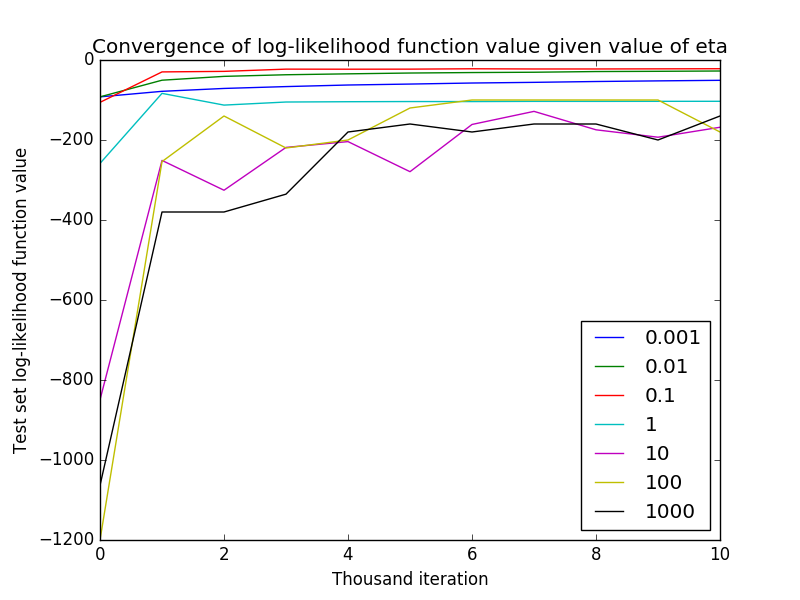
\includegraphics[scale=.5]{q1.png}
\item What was your stopping criterion and how many passes over the data did you need to complete before stopping?

\item What words are the best predictors of each class? How (mathematically) did you find them?

\item What words are the poorest predictors of classes? How (mathematically) did you find them?

\end{enumerate}

\end{document}